\section{Singapore Grand Prix}

\subsection{Circuit Analysis}

\textbf{Circuit Name:} Marina Bay Street Circuit (Singapore) \\
\textbf{Length:} 4.940 km - \textbf{Laps:} 62 - \textbf{Total Distance:} 306.143 km

\begin{figure}[H]
    \centering
    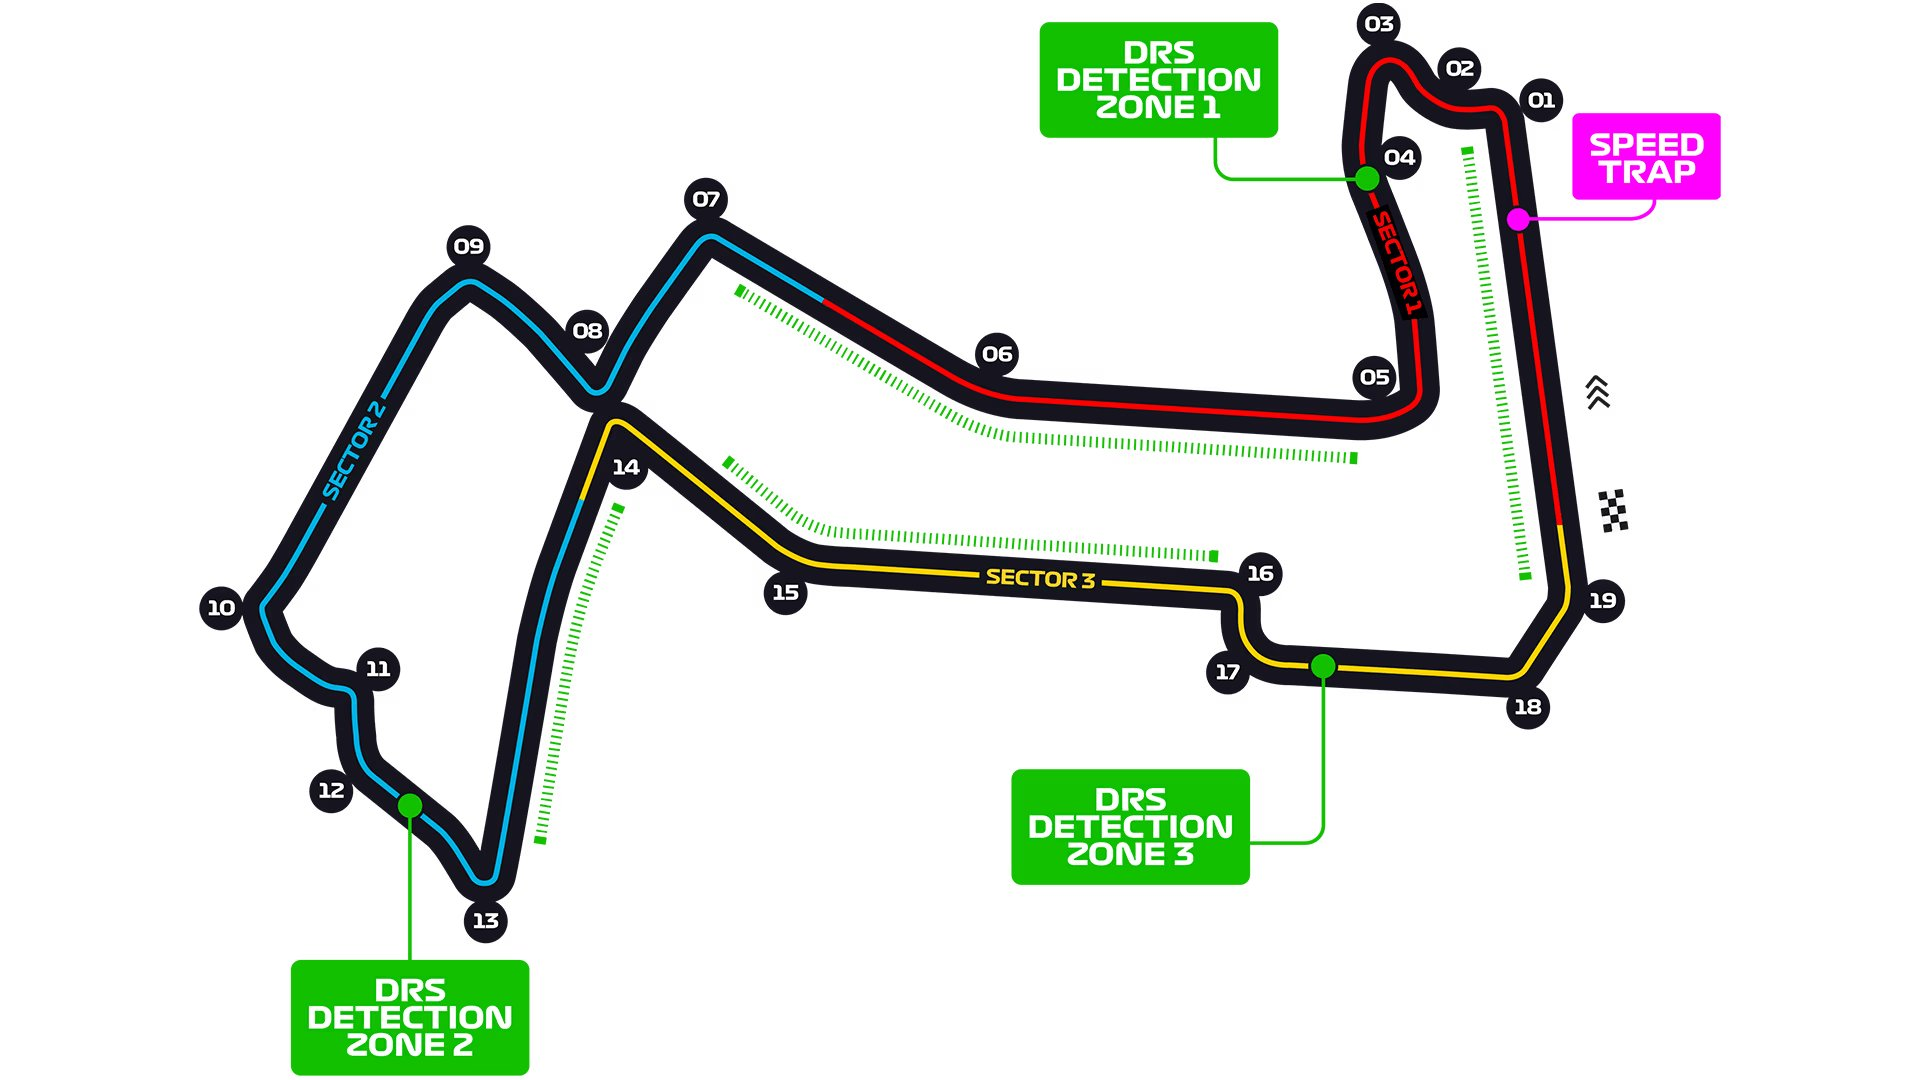
\includegraphics[width=0.75\linewidth]{images/18.Singapore_Circuit.jpg}
\end{figure}

\begin{itemize}
    \item \textbf{Lap Record} : 1:30.984 (2023, Carlos Sainz – Ferrari).
    
    \item \textbf{Number of Corners \& Key Features} : 19 turns (8 right, 11 left). \\
    Demanding street circuit with constant braking and traction zones. \\
    Night race under artificial lighting, with unique atmosphere and track conditions.
    
    \item \textbf{Braking Zones \& Traction} : Very heavy braking into Turns 1, 7 and 14. \\
    Traction out of slow corners is critical, punishing poor rear stability.
    
    \item \textbf{DRS \& Overtaking} : Four DRS zones (main straight, between Turns 5–7, before turn 14 and between Turns 14-16). \\
    Overtaking opportunities limited, mainly into Turn 7.
    
    \item \textbf{Tyre Degradation \& Strategy} : Hot and humid conditions create extreme tyre stress. \\
    Surface evolution is significant and Safety Car probability is high, influencing flexible tyre strategies.
    
    \item \textbf{Weather \& Environment} : High humidity and heat test driver endurance. \\
    Street circuit with little margin for error, walls close at every corner.
\end{itemize}

\textbf{Strategic Summary :} Marina Bay rewards qualifying, car balance in low-speed corners, and precise tyre management under extreme conditions. Track position is usually decisive due to narrow layout and difficulty overtaking.

\subsection{Race Analysis}

\textbf{Date:} 22 September 2024 — 20:00 local time 

\begin{itemize}
    \item \textbf{Qualifying Summary} : \textbf{Pole Position:} Lando Norris (McLaren) – 1:29.525 (new track record). \\
    Grid: Verstappen 2nd, Hamilton 3rd, Russell 4th. \\
    Piastri only 5th, Ferrari trapped in Q3 crash (Leclerc 9th, Sainz 10th).
    
    \item \textbf{Race Summary} : \textbf{Winner:} Lando Norris (McLaren). \\
    \textbf{Podium:} 1. Norris - 2. Verstappen - 3. Piastri. \\
    No Safety Car — first time ever in Singapore GP history. 
    
    \item \textbf{Strategies} : \\ 
    - Norris executed a clean one-stop (medium → hard), perfectly managing tyre degradation despite hot conditions. \\
    - Verstappen mirrored strategy but lacked pace to challenge. \\
    - Piastri delayed first stop, enabling overcut on Mercedes. \\
    - Ferrari split strategies: Leclerc long first stint (37 laps) on mediums before switching to hards, effective for P5. \\
    - Hamilton gambled on softs at the start, forced into early stop (lap 17) — limited to P6. 
    
    \item \textbf{Performance Trends} : \textbf{McLaren} dominant: Norris untouchable, Piastri on podium despite starting 5th. \\
    \textbf{Red Bull} showed solid race pace, but Verstappen couldn’t threaten Norris. \\
    \textbf{Ferrari} recovered well from poor grid positions, Leclerc notably effective on long stint. \\
    \textbf{Mercedes} lacked race pace to compete with McLaren and Ferrari. \\
    \textbf{Aston Martin} (Alonso) maximized potential with P8, Haas scored with Hülkenberg.
    
    \item \textbf{Championship Impact} : \textbf{Drivers:} Verstappen 331 pts, Norris 279, Leclerc 245. \\
    \textbf{Constructors:} McLaren 516, Red Bull 475, Ferrari 441, Mercedes 329.
\end{itemize}

\textbf{Key Takeaway :} Lando Norris achieved his first ever lights-to-flag victory, showcasing McLaren’s superiority in street conditions. Ferrari salvaged strong points with clever strategy, while Mercedes struggled to match rivals.

\subsection{Link \& Takeaway}

\begin{itemize}
    \item Singapore’s stop-start layout rewarded cars with strong low-speed traction and mechanical grip — McLaren’s strength in 2024. \\
    Norris dominated thanks to superior corner exit performance and tyre management in extreme heat.
    \item Ferrari’s strategic creativity (Leclerc’s long first stint) allowed recovery from poor grid positions. 
    \item Mercedes’ lack of rear grip punished them over long stints, while Aston Martin and Haas capitalized on attrition-free race. 
    \item Red Bull showed consistency but not the edge needed to beat McLaren, Verstappen’s P2 minimized losses in the title fight.
    \item With no Safety Car interventions, pure pace and tyre discipline decided the outcome — McLaren prevailed by maximizing its car’s balance in Singapore’s unique conditions.
\end{itemize}
